%%% template.tex
%%%
%%% This LaTeX source document can be used as the basis for your technical
%%% paper or abstract.

%%% The parameter to the ``documentclass'' command is very important.
%%% - use ``review'' for content submitted for review.
%%% - use ``preprint'' for accepted content you are making available.
%%% - use ``tog'' for technical papers accepted to the TOG journal and
%%%   for presentation at the SIGGRAPH or SIGGRAPH Asia conference.
%%% - use ``conference'' for final content accepted to a sponsored event
%%%   (hint: If you don't know, you should use ``conference.'')
\documentclass[tog]{acmsiggraph}

%%% Make the ``BibTeX'' word pretty...

\def\BibTeX{{\rm B\kern-.05em{\sc i\kern-.025em b}\kern-.08em
    T\kern-.1667em\lower.7ex\hbox{E}\kern-.125emX}}

%%% Used by the ``review'' variation; the online ID will be printed on 
%%% every page of the content.

\TOGonlineid{45678}

%%% Used by the ``preprint'' variation.

\TOGvolume{0}
\TOGnumber{0}

\title{Real-time Aerodynamic Sound Synthesis for Slender Objects }

\author{Jui-Hsien Wang\thanks{e-mail:jw969@cornell.edu}\\Cornell University}
\pdfauthor{Jui-Hsien Wang}

\keywords{}


\usepackage{color}
\usepackage{url}

% symbol definition
\def\p{\partial} 
\def\f{\frac} 
\def\n{\nabla} 
\def\t{\tilde}
\def\mb{\mathbf} 
\def\tb{\textbf} 
\def\etal{\emph{et al.}}
\def\tss{\textsuperscript}

\def\mbxt{(\mb{x},t)}
\def\mbtxt{(\mb{\t{x}},t)}

%%%%%%%%%%%%%%%%%%%%%%%%%%%%%%%%%%%%%%%%%
\begin{document}

%%% This is the ``teaser'' command, which puts an figure, centered, below 
%%% the title and author information, and above the body of the content.

\teaser{
  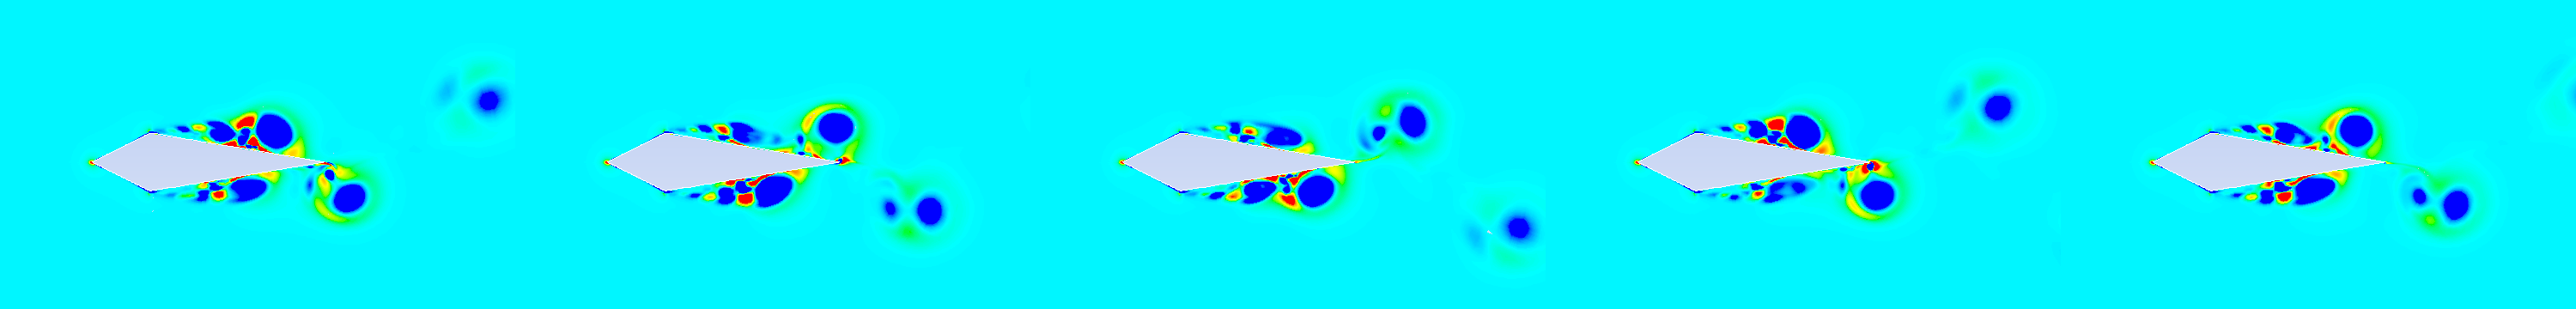
\includegraphics[height=0.8in]{./images/teaser.png}
  \caption{The vortex shedding pattern of flow over a 2D sword determines its dipole characteristics and the aerodynamic sound when swung by, say, a virtual samurai.}
}

\maketitle

\begin{abstract}

In this project, I explored the problem of real-time, physics-based aerodynamic sound synthesis for slender objects. It is largely inspired by the paper by Dobashi \etal~\cite{dobashi2003}. The aerodynamic sound when we swing a slender object, such as a stick, is originated from the complex interaction between the air flow and the stick. Sufficient spatial/temporal resolution was regarded to be essential to capture the physics and thus the characteristics of the sound generated. However, the required fluid simulation is too expensive to run at run-time audio stepping rate. To avoid such computation, I first precomputed a comprehensive database that contains relevant sound textures evaluated from high-quality grid-based fluid simulation, and then at runtime, this database is fetched and textures are blended to effectively resynthesize the aerodynamic swinging sound. Next, to increase the interactivity of the project, I interfaced the sound system with Leap Motion sensor to give real-time motion capture data. The system is proven to be quite reliable and can run at real-time even on a low-end laptop, and create realistic swinging sound. 

\end{abstract}

%  \begin{CRcatlist}
%    \CRcat{I.3.3}{Computer Graphics}{Real}{Display Algorithms}
%    \CRcat{I.3.7}{Computer Graphics}{Three-Dimensional Graphics and Realism}{Radiosity};
%  \end{CRcatlist}

\keywordlist

%% Required for all content. 

\copyrightspace


\section{Introduction} 

In games and virtual environments, accurately representing the sound of moving a slender object quickly, such as a character swinging a club, is important for story telling and the realism of the environment. However, most of the time, this sound is faked by either playing back experimentally recorded ``canned'' sound, or by using random parametric models. These models are cheap to evaluate, but they lack physical basis of how the sound is generated, and therefore can cause noticable audio-visual synchorinzation problem or need a lot of hand-tuning to ensure the quality. Dobashi \cite{dobashi2003} presented the first automated, physically-based aerodynamic sound synthesis pipeline.

This class of aerodynamic sound is generated by the fluid flow around the object, and can be described by Curle's model \cite{curle, howe2002}. Given two critical assumptions: (1) the object is acousticall compact, and (2) the listener is placed at a far-field position, the aerodynamic sound can be approximated by a dipole source, whose magnitude is govenered by the unsteady forces generated by the object placed in the flow field. Section \ref{section:curle} specifies more details on this model.

Using this model, we computed fluid flow around the object of interest and the dipole sound source function, and cached them in a database for that object for runtime evaluation. At runtime, the propagation is modeled by use of free-space Green's function, and the sound source function was used to evaluate the sound at listener's position given the motion of object. Amplitude scaling based on Curle's model and frequency scaling based on Strouhal number were implemented. Section \ref{section:sound_texture} and Section \ref{section:runtime} discuss these parts. 

Leap Motion was configured to give a run-time motion capture data, and used as the input of our sound system. The basics of this interface will be described and demonstrated in Section \ref{section:leap_motion}. 



\section{Related Work} 


\section{Curle's Model}  \label{section:curle}

For acoustically compact object and far-field listener, the sound pressure is governed by the equation \cite{curle}
\begin{align}
    p(\mathbf{q}, t) &= \f{1}{4\pi c_0 r^2} (\mb{q} - \mb{o}) \cdot \mb{g}(t-\f{r}{c_0}), \\
    \mb{g}(t) &= \f{\p}{\p t}\mb{F}(t) dS.
\end{align}
$\mb{q}$ is the listener position, and $\mb{o}$ is the object center position. $c_0$ is the speed of sound, $r$ is the distance between listener and object center, and $\mb{F}$ is the aerodynamic forces of the object in the texture domain, precomputed in the fluid simulation. Given this model, we can statically sample and cache the function $\mb{g}$ at different inflow speed and directions for a given object, and only evaluate the sound propagation at runtime. The runtime cost would be a data-fetching process, and a few flops to decide the position and direction of the object with respect to the listener in order to scale the sound amplitude and time delay.


\section{Sound Texture Database Construction}  \label{section:sound_texture}

The sound source function, $\mb{g}$, can be precomputed in a fluid simulation. I used proprietary finite-volume solver Ansys Fluent to do the computation. The object being sampled was placed in a virtual wind tunnel and rotated with $5$ degree interval to sample the sound source function for every inflow direction. To shorten this preprocess, the following identities are used
\begin{itemize}
    \item [(1)] The amplitude of the dipole sound scales linearly with inflow speed in the log-space. That is, $|p_v| = (v/v_0)^\alpha |p_{v_0}|$. $\alpha=6$ is the coefficient Dobashi used, but I found that $\alpha \approx 2$ works better because the high coefficient gives too wide the dynamic range.
    \item [(2)] The frequency of the dipole sound scales linearly with inflow speed. The physical argument here is based on the Strouhal frequency, $St = f D/v$, where $St$ is the Strouhal number, $D$ is the diameter of the cylinder, and $f$ is the frequency. For a wide range of Reynold's number ($Re=100 \sim 1E6$), the Strouhal number stays roughly constant for cylinder ($St_{cylinder} \sim 0.21$) and therefore for the same object, the frequency scales linearly with inflow velocity. Linear interpolation was applied to sound textures to first upsample it to avoid artifacts when we scale the textures. 
    \item [(3)] For inflow with non-zero incidence angle, the sound is approximately equal to the sound created by inflow speed scaled by the geometric factor. Therefore, all the inflow directions at runtime were projected to the normal direction of the object before the sound source function was evaluated. $sound(v_\theta) \approx  sound(v_{\|})$, $v_{\|} = v \cos\theta$.

\end{itemize}


\section{Runtime Considerations} \label{section:runtime}

One of the big problems I encountered when implementing this paper was how to do the real-time audio rendering properly, the discussion of which is missing from the paper. There were two main problems associated to it: (1) the time-scale mismatch in motion capture refresh rate and audio stream sampling rate can cause severe ``clicking'' sound when scaling the textures or jumping between textures. (2) the audio underrun caused by improper thread priority for audio callback and high motion capture latency.

The clicking problem (either caused by resampling the texture in the amplitude/frequency shifting or jumping between textures) can be resolved by requesting an optimum buffer size. To avoid audio glitch, the audio interface (I use portaudio) reduces the number of audio callbacks by requesting an audio buffer when the audio stream is opened. The size of the buffer can be fixed or adaptive, depending on the hardware implementation and the application (for example, the CoreAudio framework in MacOS is well written, and can largely reduce the latency). What I did to resolve the clicking was to enforce the motion-capture data to be sent only when audio callback happens, and then linearly blend between the two states of motion data (sound amplitude/frequency). I found that the buffer size of $\sim100$ works the best. If the buffer is too large, the motion-capture data is updated infrequenctly and the playback will sound sluggish; whereas if its too small, then the buffer doesn't have enough time to blend the textures and clicking will occur. Note that this number is roughly the ratio between audio sampling rate (for most of them is $10000$Hz) and motion-capture update refresh rate (at around $100$Hz).

The audio underrun can happen when the buffer cannot be properly filled in the requested time frame, and portaudio has no choice but to fill the buffer with zeros. This problem can be severe, but can be resolved by requesting a high-priority thread to the audio callback and another high-priority thread for motion-capture. Also, unbounded time operations such as file I/O should be completely avoided or minimized in the audio callback. For the same reason, the sound textures should all be loaded when the program starts, to avoid unnecessary underrun at the cost of higher memory footprint.



\section{Real-time Motion Capture} \label{section:leap_motion}


\subsection{Integration with the sound system}

The motion capture system should input the state of the object in order to fetch the database. Position, speed and orientation are the required metrics to determine the sound state.  



\subsection{Using mouse cursor} 



\subsection{Using Leap Motion}



\section{Result} 

\subsection{Implementation Details} 




\section*{Acknowledgements}



% Problem geometry, meshing bala

% Fluent simulation setup 




% \section{The Basics: General Organization}
% 
% Your content should have the following elements, in this order:
% \begin{itemize}
% \item title, author, and affiliation information
% \item abstract
% \item CR categories *
% \item keywords *
% \item body of the content
% \item bibliography
% \end{itemize}
% 
% CR categories and keywords are required for Technical Papers and
% Technical Briefs, and optional for all other types of content. The
% \LaTeX{} and Word templates faithfully implement the formatting
% specifications in this document, and the sample PDF documents can be
% used as visual examples for organization and layout.
% 
% \section{The Basics: Page Size and Columns}
% 
% Your content should be formatted on a US Letter (8.5 inches wide by 11
% inches tall) page size. Please make sure you.re not working on an A4
% page size. Page margins should be set at 0.75 inches on the right,
% left, and top, and one inch at the bottom. Two columns should be used
% throughout your content, except for the title, affiliations, and large
% images or tables which span both columns.
% 
% To summarize, here are the basic page specifications: 
% \begin{itemize}
% \item page size: 8.5 inches wide by 11 inches wide (not A4)
% \item top margin: 0.75 inches
% \item right margin: 0.75 inches
% \item left margin: 0.75 inches
% \item bottom margin: 1 inch
% \item number of columns: 2
% \item column width: 3.3 inches
% \item column height: 9.25 inches
% \item column gutter: 0.33 inches
% \end{itemize}
% 
% \section{The Basics: Typefaces, Paragraphs, and Line Spacing}
% 
% Please use a serif (Times, Times New Roman, etc.) typeface for the
% body of your content. This serif typeface should be used for
% everything except the title of your content and section headings,
% which should be set in a sans-serif (Helvetica, etc.) typeface.
% 
% Your content should be prepared with 9-point text and 10-point line
% spacing. This includes the references section. Do not reduce the
% typeface size or the line spacing of any part of your content, in an
% effort to fit more into a specific number of pages. 
% 
% All typefaces used in your content must be embedded in the PDF you
% create. 
% 
% Paragraphs are prepared without any indentation on the first line, and
% with a 10-point-tall space between paragraphs.
% 
% Please do not add page numbers to your content. They will be added
% during production.
% 
% \section{The Basics: Title, Author, and Affiliation Information}
% 
% The title, author, and affiliation information should be centered
% above the body of your content. The title should be set in a 14-point
% bold sans-serif typeface with 18-point line spacing. The author and
% affiliation information should be set in a 10-point serif typeface
% with 12-point line spacing.
% 
% The title should be appropriately capitalized. ``All caps'' is not
% appropriate. The following link provides assistance with appropriate
% capitalization:
% 
% {\small\url{http://www.grammarbook.com/punctuation/capital.asp}}
% 
% Affiliations should include your educational institution or employer's
% name, and a valid e-mail address.
% 
% \section{The Basics: Section Headings}
% 
% Section headings should be set in a 10-point bold sans-serif typeface
% and numbered - ``1'', ``2'', and so on. Subsection headings should be
% set in a 10-point bold sans-serif typeface and numbered - ``1.1'',
% ``1.2'', and so on. Subsubsection headings should be set in a 10-point
% italic sans-serif typeface and numbered - ``1.2.1'', ``1.2.2'', and so
% on. A 10-point-tall space should separate a section heading and the
% next paragraph.
% 
% \section{Abstract, Keywords, and CR Categories}
% 
% Your content should begin with an abstract of about 150 words,
% describing the work and its contribution to the field.
% 
% Authors of technical papers and technical briefs must also provide a
% set of user-generated keywords and a selection of CR categories, from
% the following link:
% 
% {\small\url{http://www.acm.org/about/class/1998/}}
% 
% Authors of other types of content may include CR categories and
% keywords at their discretion.
% 
% \section{ACM Rights Management Text}
% 
% You are required to leave a blank space at the base of the left column
% on the first page of your content for the ACM rights management
% text. This blank space will be one column wide, and one inch tall for
% all types of content except technical papers accepted to our annual
% (SIGGRAPH and SIGGRAPH Asia) conferences. In this case, the space must
% be 1.5 inches tall. (These technical papers are accepted as articles
% in the ACM ``Transactions on Graphics'' journal, and the rights
% management text is slightly different, and occupies more space.)
% 
% \section{Figures and Tables and Captions}
% 
% Figures and tables can span one or both columns. Captions for figures
% should be centered underneath the figure. Captions for tables should
% be centered above the table.
% 
% \begin{table}[ht]
%   \centering
%   \caption{A simple table.}
%   \begin{tabular}{|r|l|}
%     \hline
%     7C0 & hexadecimal \\
%     3700 & octal \\ \cline{2-2}
%     11111000000 & binary \\
%     \hline \hline
%     1984 & decimal \\
%     \hline
%   \end{tabular}
% \end{table}
%   
% Please use 9-point bold serif type for the caption title, and 9-point
% serif type for the caption text (both on 10-point line spacing).
% 
% \section{Citations and References}
% 
% \subsection{Citations}
% 
% The SIGGRAPH citation format is the ``author year''
% format~\cite{Pellacini:2005:LAH}. The year is separated from the
% author by a single space~\cite{yee:2000:ssa}. Two authors are
% separated by the word ``and''~\cite{parke:1996:CFA}. More than two
% authors are represented by the primary author and ``et al.''~\cite{levoy:2000:TDM}.
% 
% Multiple citations at a single point in the content are separated by
% semicolons~\cite{levoy:2000:TDM,sako:2001:SSB}.
% 
% When the last name of the cited author is part of the text, it may be
% omitted from the citation: ``\ldots as shown in Fedkiw et
% al.~\shortcite{fedkiw:2001:VSO}, the coefficient remains\ldots''
% 
% \subsection{References}
% 
% The reference list, or bibliography, must be unnumbered, alphabetized
% by the primary author's last name, followed by the year of publication
% and other identifying information (article title, journal title,
% volume, number, etc.). Author names are arranged as ``last name,
% initials.'' The page number, if any, is the last piece of information
% in the reference.
% 
% The first line of each entry in the bibliography has no
% indentation. The second successive lines has a 2em
% indentation. 
% 
% Please use 9-point serif type, with 10-point line spacing, for each
% entry in the bibliography, with a single blank line between each
% entry. 
% 
% Journal, book, thesis, and conference proceedings titles are set in an
% italic serif type. {\sc Author names should be typeset in a ``Small
% Caps'' typeface.}
% 
% \section{Third-Party Material}
% 
% If you are using third-party material in your content - that is,
% material which you or your co-authors did not create - you need to
% clearly identify it as such in the material itself or in the 
% content's caption, as shown in Figure~\ref{fig:ferrari}.
% 
% \begin{figure}[ht]
%   \centering
%   \includegraphics[width=3.0in]{images/ferrari_laferrari}
%   \caption{Ferrari LaFerrari. Image courtesy Flickr user ``gfreeman23.''}
%   \label{fig:ferrari}
% \end{figure}
% 
% ACM's policy on third-party material can be found at the following link:
% 
% {\small\url{http://www.acm.org/publications/third-party-material}}
% 
% \section{``Artistic Images'' and Copyright Transfer}
% 
% ACM's rights management policy mandates that if copyright is
% transferred to ACM, and authors wish to retain copyright of one or
% more of their own images or figures in the content, they can identify
% them as ``artistic images'' by including the author's copyright notice
% in the image itself or in the caption.
% 
% (Please note that only technical papers and technical briefs have
% copyright transfer as an option. All other forms of content have
% permission and licensing options, but not copyright transfer.)
% 
% \section{Author-Prepared Versions of Final Content}
% 
% ACM's rights management policy provides for author-prepared versions
% of final content to be made available on the author's personal or
% employer's web site for distribution.
% 
% The author is responsible for creating the article-specific notice and
% making it part of the PDF. The following is an example of such a
% notice. Yours will have the year, publication, and article DOI
% information specific to your final content.
% 
% \texttt{\small(c) 2009 ACM. This is the author's version of the work. It is posted here by permission of ACM for your personal use. Not for redistribution. The definitive version was published in ACM Transactions on Graphics 28(3), August 2009. http://doi.acm.org/10.1145/1576246.1531329.}
% 
% \section{Application-Specific Notes}
% 
% \subsection{\LaTeX}
% 
% The ``acmsiggraph'' \LaTeX{} class will faithfully implement the formatting specifications found in this document. Please look at the ``template.tex'' file that accompanies the \LaTeX\ and \BibTeX\ class files, noting these points:
% \begin{itemize}
% \item In order to leave the correct amount of space clear for the rights management text, you must do two things: 
% \begin{enumerate}
% \item Use the proper parameter to the \cs{documentclass} command at the top of your source file: use ``tog'' for technical papers accepted to our annual events and published as TOG articles, and use ``conference'' for all other types of content. The parameter determines the amount of space left clear for the rights management text.
% \item Use the \cs{copyrightspace} command. It should be placed immediately before the first section of your paper.
% \end{enumerate}
% If you do not use any parameter to the \cs{documentclass} command, and use the \cs{copyrightspace} command, you'll end up with much more blank space than you want or need.
% 
% \item Many authors like to have a large image - called a ``teaser'' image - after the title, author, and affiliation and before the body of the paper. There is a command - \cs{teaser} - which can be used to place such an image. (As has been done in this example document.) Under certain circumstances, the space left clear for the rights management text will move to the base of the right column on the first page. This is acceptable.
% \item Use the \cs{keywords} command to define your own keywords, and the \cs{keywordlist} command to prepare and print that block of text.
% \item Use the \cs{CRcatlist} environment and the \cs{CRcat} command to define the CR categories appropriate for your paper.
% \item There are also ``review'' and ``preprint'' variations of this document class, to be used for material submitted for review, and accepted content to be distributed as a ``preprint.'' These variations have special commands associated with them; see the ``template.tex'' file for more information.
% \end{itemize}
% 
% \subsection{Microsoft Word}
% 
% The ``acmsiggraph.docx'' file will faithfully implement the formatting
% specifications found in this document.
% 
% An appropriately-placed column break is one way to leave the right
% amount of space for the rights management text.
% 
% \section{Proceedings Production}
% 
% Your final content will be checked and, if found acceptable for publication, will have the appropriate page header and footer information and ACM rights management text added to it. 
% 
% If your final content is not acceptable for publication - for example, unembedded typefaces, missing required elements, or modification of the format - you will be directed to correct these issues and submit a new version of your final content as soon as possible.
% 
% \section{Contact Information}
% 
% If you have questions or suggestions regarding this document, please
% contact Stephen Spencer at ``spencer@cs.washington.edu''.
% 
% 
% To Robert, for all the bagels.

\bibliographystyle{acmsiggraph}
% \nocite{*}
\bibliography{reference}
\end{document}


